

\documentclass[12pt]{article}
\usepackage[utf8]{inputenc}
\usepackage{marvosym}
\usepackage{color}
\usepackage{amssymb,amsmath,amstext,amsfonts,amsthm}
\usepackage[gen]{eurosym}
\usepackage{fancyhdr,fancyvrb}
\usepackage{latexsym}
\usepackage{graphicx}
\usepackage{placeins,lscape}
\usepackage[normalem]{ulem}
\usepackage{cancel}
\usepackage{chngcntr}
\usepackage{footnote}
\usepackage{caption}
\usepackage{array}
\usepackage{rotating}
\usepackage{dcolumn }
\captionsetup[figure]{labelfont=bf}
\captionsetup[table]{labelfont=bf}
\usepackage{subfigure}
\usepackage{colortbl}
\newcommand{\gray}{\rowcolor[gray]{.90}}
\setlength{\parindent}{0cm}
\renewcommand{\rmdefault}{ptm}
\renewcommand{\thesubsection}{\thesection.\alph{subsection}}
\usepackage{alltt}
\usepackage{lscape}
\usepackage{dcolumn}
\usepackage{booktabs,caption,fixltx2e}
\usepackage[flushleft]{threeparttable}
\usepackage{float}
\usepackage{graphicx}
\captionsetup[figure]{skip=0pt}
\usepackage[paper=portrait,pagesize]{typearea}
\usepackage{setspace}
\usepackage{lmodern}
\DeclareMathOperator{\EX}{\mathbb{E}}% expected value
\setcounter{MaxMatrixCols}{10}
\setcounter{tocdepth}{5}
\setcounter{secnumdepth}{5}
\oddsidemargin 0cm \evensidemargin 0mm \topmargin -20mm \textwidth 16.5cm \textheight 24cm
\setlength{\parskip}{5pt}
\renewcommand{\topfraction}{.85}
\renewcommand{\bottomfraction}{.7}
\renewcommand{\textfraction}{.15}
\renewcommand{\floatpagefraction}{.66}
\renewcommand{\dbltopfraction}{.66}
\renewcommand{\dblfloatpagefraction}{.66}
\setcounter{topnumber}{9}
\setcounter{bottomnumber}{9}
\setcounter{totalnumber}{20}
\setcounter{dbltopnumber}{9}
\newtheorem{taable}{Table}
\renewcommand{\baselinestretch}{1.5}
\linespread{1.5}
\usepackage{listings}
\inputencoding{latin1}
\inputencoding{utf8}
\newcommand{\vect}[1]{\boldsymbol{#1}}
%\usepackage{tgpagella} % text only
\usepackage{mathpazo}  % math & text


%%%%%%%%%%%%%%%%%%%% CITE %%%%%%%%%%%%%%%%%%%%%%%%%%%%
\usepackage{hyperref}
\hypersetup{
	colorlinks=true,
	linkcolor=red,
	filecolor=magenta,      
	urlcolor=cyan,
}
\usepackage[round, sort, authoryear]{natbib}
\bibliographystyle{apalike}
\hypersetup{citecolor=red}
\usepackage[numbib]{tocbibind}

%%%%%%%%%%%%%%%%%%%%%%%%%%%%%%%%%%%%%%%%%%%%%%%%%%%%%


\title{Dealing with the Dutch Cap Bonus \thanks{Acknowledgments: All remaining errors are ours.}}

\author{Ata Bertay \thanks{%
		Sabanci Business School. Sabanci University.}   \ \   José Gabo Carreño\thanks{%
		Department of economics. Tilburg University} \ \ \ Harry Huizinga\footnotemark[3] \\  Burak Uras\footnotemark[3] \ \ Nathanael Vellekoop\thanks{Department of economics. University of Toronto.} }


\date{\today}



\begin{document}

\maketitle

%\centerline{[\textbf{\textit{PRELIMINARY VERSION}}]}
\begin{abstract}

We use a ...

\textbf{Keywords}: ...

\end{abstract}
\vspace{1cm}


\newpage

%===================================================================================
\section{Introduction}
%===================================================================================

[NICE INTRO ABOUT THE FINANCIAL CRISES, BANK REGULATION, AND SALARIES] \\

This paper evaluates the Dutch bonus cap (DBC), which introduced a 20\% bonus cap for financial undertakings in 2016. We combine administrative data to measure program exposure and savings outcomes for all workers in the banking industry. We use difference-in-difference 
design to estimate the effect of the DBC on savings. Our difference-in-difference design compares group of workers at the same point in time whose exposure to the program differs. We define policy exposure based on the salary in 2012. Workers with a low salary in 2012 serve as ``control group'' because the policy does not induce many banks to change their salary. \\

We present several findings. First, the policy proved effective at decreasing the salary growth at the top-decile. Second, workers at the top- decile changed the wage composition...


\newpage
%=====================================================================================
\section{Literature Review} \label{literature_review}
%=====================================================================================

\subsection{Results in the literature related the bonus cap}

\begin{itemize}		
	\item \citet{colonnello2018effectiveness}:  A very good starting point to start working on this topic. They classified bankers with a binding bonus cap as treated.  They then run a DiD where the outcome is risk-taking.  They find mixed evidence. He also seems that literature does not have evidence for the full economy to study the impact of bonus cap in the finance industry (except by \citet{abudy2020executive}).   
	\item \citet{efing2018bank}: They argue that risk sharing motivates the bank-wide structure of bonus pay. This is paper is interesting because they have employee-employer data. Yet do not have advantage of any quasi-experiment but the financial crisis.  They document very interesting fact that we can also look at. This paper is motivated in the theoretical work of \citet{thanassoulis2012case}.
	\item \citet{abudy2020executive}: They exploit a the same quasi-experiment than us.  They find that compensation
	contracts can be set in a way that does not maximize firm value. Yet, they have information at firm level. We have information employeer-employee. 
	
\end{itemize}


\subsection{Results related to fix/variable proportion of salary}

\begin{itemize}	
	\item ...
	
\end{itemize}




\subsection{Methods: Diff-in-Diff}

\begin{itemize}	
	\item \citet{berger2020stimulating}: They document the effect of the FTHC on home sales. Our difference in differences design compares ZIP codes at the same point in time whose
	exposure to the program differs. We define program exposure based on the number of potential first-time home buyers in a ZIP code. ZIP codes with few potential first-time homebuyers serve as a “control group” because the policy does not induce many people to buy in these places. We measure exposure as
	the year-2000 share of people in a ZIP code who are first-time homebuyers. 
	
	\begin{figure}[H]
		\centering
		\caption{Figure 5 from \citet{berger2020stimulating}.}
		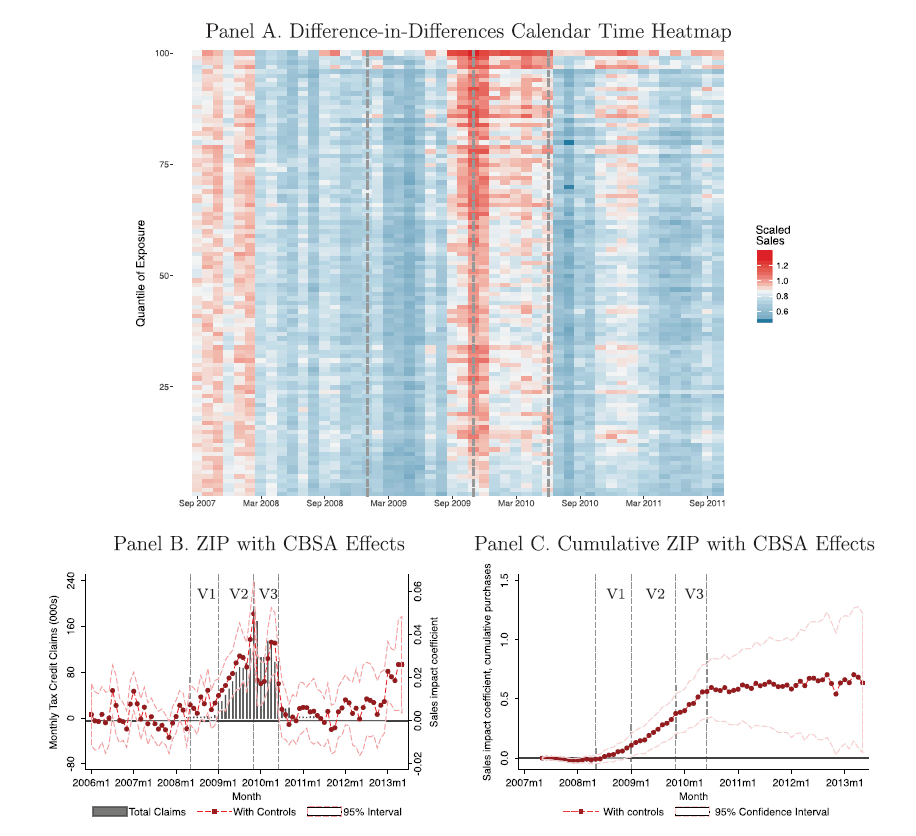
\includegraphics[width=0.7\linewidth]{figure5_empirical_approach}
		
		\label{fig:figure5empiricalapproach}
	\end{figure}
	
\end{itemize}



\newpage
%=====================================================================================
\section{Bonus cap in the Netherlands} \label{bonus_cap}
%=====================================================================================



\begin{itemize}
	\item \textbf{On 5 March 2013} the EU finance ministers decided that European banker's bonuses should be capped at a maximum of 100\% their base salary, rising to 200\% if shareholders explicitly agree. 
	\item \textbf{On 26 November 2013}, the Dutch government published a draft legislative proposal in which it introduced a 20\% bonus
	cap for financial undertakings. 
	\item \textbf{On 7 February 2015} was introduced the Dutch Act on the Remuneration Policies Financial Undertakings (Wet beloningsbeleid financiële ondernemingen, the ``Act'').
	\item The central point of the Act is the 20\% bonus cap: a financial undertaking cannot pay any person ``working under its responsibility'' variable remuneration that exceeds 20\% of the fixed remuneration on an annual
	basis.\footnote{Remuneration is either fixed or variable. The Act has a broad definition of variable remuneration, ``all remuneration that is not fixed remuneration'', whereas the definition of fixed remuneration is ``the part of the total remuneration that consists of unconditional financial or non-financial payments''.}
	\item Employees may be awarded a bonus exceeding 20\% of the fixed pay in 2015 if such award stems from an obligation existing prior to 1 January 2015. The Minister of Finance has made it clear that this exception only applies to 2014 performance bonuses that are awarded in 2015.\textbf{ As from 1 January 2016, any bonus award is subject to the rules of the Act.}
	\item The Act applies to financial undertakings (financiële ondernemingen) with their official seat in the Netherlands and their subsidiaries (including subsidiaries abroad).
	\item The definition of ``financial undertaking'' is very broad and includes, amongst others, banks, insurers, investment firms, fund managers, payment services providers, custodians and premium pension institutions (PPIs). \textbf{However, the bonus cap does not apply to:}
	\begin{itemize}
		\item Pension funds.
		\item Asset managers.
		\item  Branches of banks and investment
		firms located in the Netherlands with a
		‘mother firm’ in another member state
		of the European Union and which are
		subject to the Capital Requirements
		Directives IV (CRD IV).
		\item Investment institutions and institutions
		for collective investment in securities.
		These institutions should invest on their
		own account with their own resources
		and capital, and have no external
		customers.
	\end{itemize}
	
\end{itemize}


\newpage
%=====================================================================================
\section{Data} \label{data}
%=====================================================================================


[DESCRIPTION OF THE DUTCH DATA]

Our data allows us to decompose the worker's pay into base salary, special remuneration,\footnote{This concerns, for example, holiday allowance, end-of-year benefits, performance benefits, bonuses and profit distributions. The special rewards do not include: contributions to savings schemes, termination benefits, health insurance allowances and wages for overtime.} extra salaries,\footnote{Regarding the extra salary, it is not clear if this item should be considered fixed or variable. We can show that banks used it to compensate bankers in 2014.} and overtime worked hours. \\


\subsection{Evidence looking at the data}
	
	\begin{itemize}
		\item Regarding the VPR dynamics, special remuneration over basic wage, we have the following. 
		\begin{enumerate}
			\item Banks: While the VPR jumped in 2013, it decreased in 2014 to a level lower than 2012. After 2014, the VPR has remained in approximately the same level than 2014. Therefore, the dynamic are related to the announcement, but not to the start of the regulation.\footnote{The lower VPR is explained by a lower special remuneration. The basic wage has grown constantly over time. } \textbf{Who were more affected?}  Worker on the top decile according to the gross wage. It seems that they were also more prone to leave the finance industry. 
			\item Insurance: We so see a change in 2015 (lower value) when compared to 2012 or 2013.
			\item Pensions: We do see a change in 2015/2016. It does not seem consistent with the timing of the regulation.  
			%\item Banks: The VPR in 2012 cannot help to explain who were treated in 2014. Two reasons: (1) the VPR is not related to the gross wage. Everyone can get a high VPR in the finance industry; (2) The VPR in in fact variable. Getting a high VPR in 2012 does not predict a higher VPR in 2014. 
			%\item Small exercise. We consider workers staying in the finance industry over the period 2012-2014. We classify workers in deciles by using the gross wage in 2012. We calculate the VPR change between 2012 and 2014. We do see that workers at the top deciles were more affected by the dutch cap. They suffered a 2.5\% media reduction of the VPR between 2012 and 2014. We also observe a reduction in the gross wage of workers at the top deciles. 
			%\item It is important to note that there is not a clear relationship between the VPR and the gross wage. So, it is not possible to anticipate
			%\item Continuing the exercise, we check how many workers were still employed in 2015. Remember that we are considering workers stayed in the finance industry over the period 2012-2014. We do see that 20\% of workers at the top decile left the finance industry. Contrarily, we see that just 10\% of worker left at lower deciles. 
			
		\end{enumerate}
	\item We compare group of workers by the exposition to the cap. We define policy exposure based on the gross wage decile in 2012. 
	\item Banks: We observe that top decile was the most affected regarding special remuneration. This variables has not recovered over time. We also observe a rapid growth of the basic wage for the top-decile that make the gross wage to growth just after 2014. 
	\item We do not see a big impact on employment at the top decile. Yet, we observe that an important number of workers left the banking industry at the end of 2013 (all of them did much worse than their peers in terms of the gross wage). I could not find much more about this. 
	
		
	\end{itemize}
	






\newpage
%=====================================================================================
\section{Estimation Methods} \label{estimation_methods}
%=====================================================================================

To estimate 

\newpage
\section{Concluding remarks} \label{conclusions}

This paper has analyzed the 


\newpage





\setcitestyle{numbers}
%\bibliographystyle{apalike}
\bibliography{BCHUV_cap_biblio_2022}





\newpage
























\appendix
\renewcommand{\thefigure}{A\arabic{figure}}
\renewcommand{\thetable}{A\arabic{table}}
\renewcommand{\theequation}{A\arabic{equation}}

\setcounter{figure}{0}
\setcounter{table}{0}

%EXAMPLE OF HOW TO USE SUBFIGURE (DO NOT DELETE)
%==============================================================================
%\begin{figure}[H] 
%\centering 
%\caption{Wage rigidities and welfare under CM2016's loss function: currency union versus inflation targeting.} \label{fig:gm2016_welfare_losses} 
%\subfigure[Demand shocks]{% 
%	\includegraphics[width=.45\textwidth]{wealth_loss_infl_vs_peg_z_shock_CM2016} } 
%\quad
%\subfigure[Technology shocks]{\includegraphics[width=.45\textwidth]{wealth_loss_infl_vs_peg_a_shock_CM20%16} } 
%
%\end{figure}
%==============================================================================


\newpage
\KOMAoptions{paper=portrait,pagesize}
\recalctypearea

\newpage
\begin{center}
    \textbf{APPENDIX}
\end{center}

\section{XXXX}


\end{document}
